\chapter{Die Data Warehousing Workbench}
\label{Abschnitt:Motivation}

\begin{figure}[H]
    \centering
    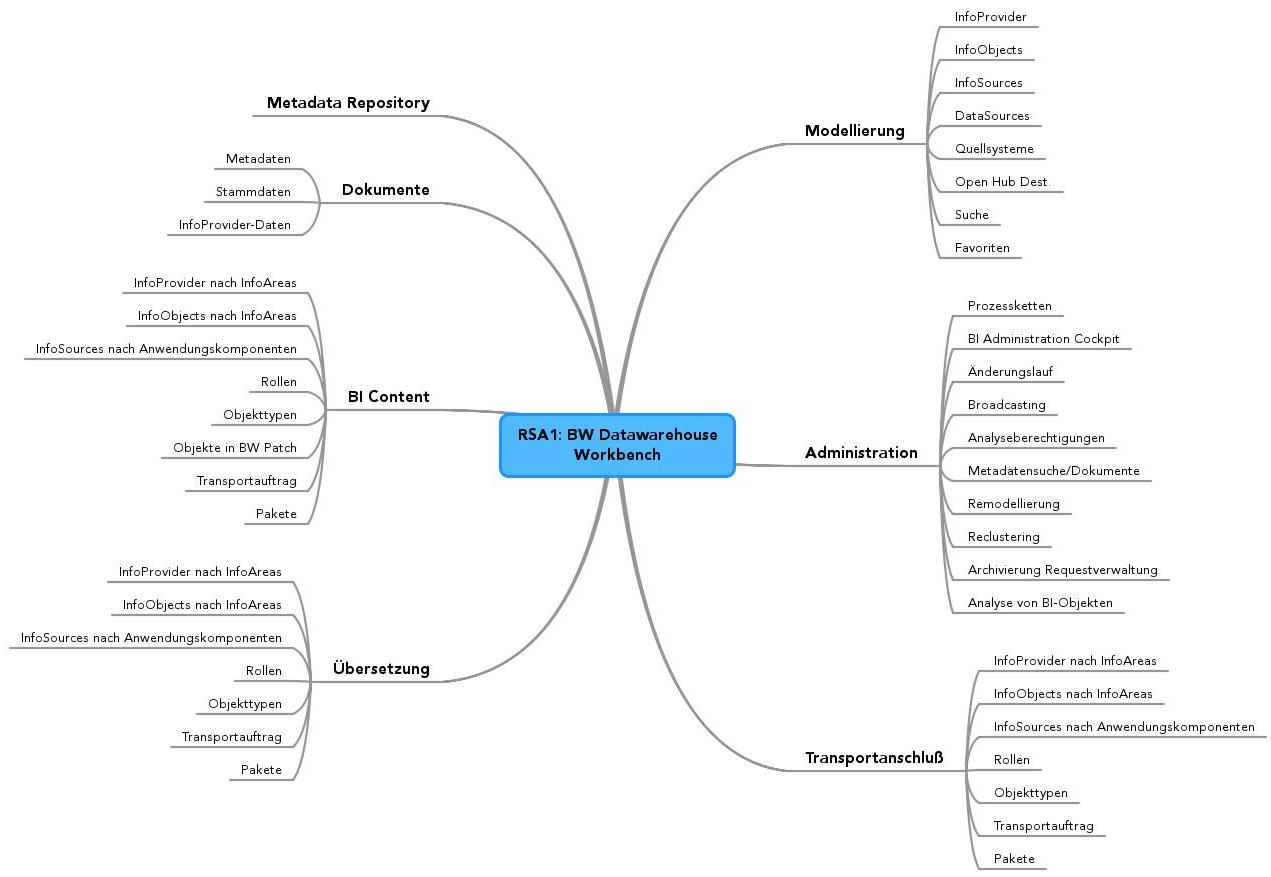
\includegraphics[width=1\textwidth]{files/RSA1Mindmap}
    \caption{Übersicht über RSA1}
    \label{pic:RSA1}
\end{figure}


Die \textit{ Data Warehousing Workbench} lässt sich in die folgenden sieben Module unterteilen, welche in \textbf{Abb. \ref{pic:RSA1}} in einem übersichtlichen Diagramm aufgelistet sind.\\

\begin{description}
\item[Modellierung:] Dieses Modul dient zur Modellierung von Daten und es werden verschiedene BI-Objekte bereitgestellt, welche zur Integration, Transformation, Konsolidierung, Bereinigung und Ablage von Daten genutzt werden können. Die verfügbaren BI-Objekte sind folgende:
\begin{itemize}
\item \textbf{InfoProvider:}
Oberbegriff für BI-Objekte, in die Daten hinein geladen werden können, bzw. Sichten auf die bereits geladenen Daten darstellen. Diese Daten können zu einem späteren Zeitpunkt mit dem BEx Query-Designer ausgewertet werden.

BI-Objekte sind zum einen Objekte, in denen Daten physisch vorhanden sind, wie InfoCubes, DataStore-Objekte und InfoObjects (Merkmale mit Attributen oder Texten). Zum anderen zählen dazu auch Objekte, die keine physische Datenablage darstellen, wie InfoSets, VirtualProvider und MultiProvider.

\item \textbf{InfoCubes:}
Spezifischere Variante eines InfoProviders.
Ein InfoCube beschreibt einen in sich geschlossenen Datenbestand z.B. eines betriebswirtschaftlichen Bereichs. Dieser Datenbestand kann mit dem BEx Query-Designer ausgewertet werden.

Ein InfoCube besteht aus relationalen Tabellen, die nach dem Sternschema zusammengestellt sind: eine große Faktentabelle im Zentrum und mehrere sie umgebende Dimensionstabellen.
Sie werden aus InfoSources oder anderen InfoProvidern mit Daten versorgt und stehen im Anschluss für das Reporting bzw. die Analyse zur Verfügung.

\item \textbf{InfoSources}
Es wird zwischen zwei Arten von InfoSources unterschieden:
-InfoSources mit \textit{flexibler} Fortschreibung
-InfoSources mit \textit{direkter} Fortschreibung

Diese bestehen aus einer Menge von Informationen, die zusammengefasst und bereitgestellt werden. Diese Informationen können Bewegungsdaten und Stammdaten sein.

Beide Arten transformieren die geladenen Daten durch Übertragungsregeln, die vorher definiert werden müssen. Die Regeln beziehen sich auf die Kombination von einer InfoSource und einem Quellsystem bzw. auf jedes InfoObjekt. Eine InfoSource kann mehrere InfoProvider mit Daten beliefern und selbst von mehreren Quellsystemen mit Daten versorgt werden.
Bei der flexiblen Fortschreibung werden die Daten in die Datenziele (InfoCube, DataStore-Objekt, Stammdaten) geladen.
Bei der direkten Fortschreibung können Stammdaten eines InfoObjects direkt in die Stammdatentabelle fortgeschrieben werden (dies ist nur mit Stammdaten möglich).

\end{itemize}
Die Grafische Oberfläche ist in  \textbf{Abb. \ref{pic:Modellierung}}  zu sehen.
\begin{figure}[H]
    \centering
    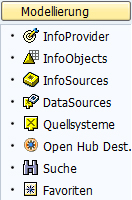
\includegraphics[width=0.2\textwidth]{files/Modellierung}
    \caption{Das Modellierungsmenü}
    \label{pic:Modellierung}
\end{figure}
\item[Administration:] Hier befindet sich eine Ansicht für die verschiedensten Prozessketten, sowie das BI Administration Cockpit. Jenes wird verwendet, um die Performance von BI-Systemen zu überwachen. Es liefert einen zentralen Einstiegspunkt, sowie ein real-Time Monitoring und verschiedene Laufzeitstatistiken. Es bietet Zugriff auf Berichte und Anwendungen, die den Anwender bei der Ermittlung und Analyse von Problemen unterstützt. Es können BI-Objekte nachverfolgt und die Performance von BI-Aktivitäten optimiert werden.
Die Grafische Oberfläche ist in  \textbf{Abb. \ref{pic:Administration}}  zu sehen.
\begin{figure}[H]
    \centering
    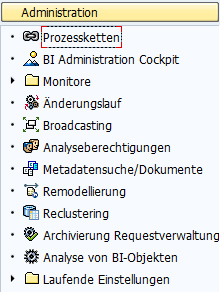
\includegraphics[width=0.4\textwidth]{files/Administration}
    \caption{Das Administrationsmenü}
    \label{pic:Administration}
\end{figure}
\item[BI Content:] Die Struktur der verarbeiteten Geschäftsinformationen eines Unternehmens kann zu Auswertungszwecken im BI Content modelliert werden. Diese Modelle setzen sich aus verschiedenen Metadaten-Objekttypen zusammen. Hierbei werden vorkonfigurierte zur Analyse betriebswirtschaftlicher Fragestellungen verwendet. Wichtig hierbei ist, dass die Erzeugung, Verwendung, Überarbeitung und der Transport der BI-Objekte konsistent gehalten wird. Ein enthaltenes Konzept ist das \textit{BI-Versionskonzept} und eine Hauptfunktionalität ist die Übernahme von neuem BI Content in das Produktivsystem.
Die Grafische Oberfläche ist in \textbf{Abb. \ref{pic:BIContent}} zu sehen.
\begin{figure}[H]
    \centering
    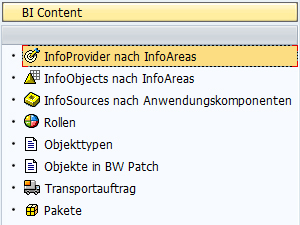
\includegraphics[width=0.45\textwidth]{files/BIContent}
    \caption{das BI Content Menü}
    \label{pic:BIContent}
\end{figure}
\item[Transportanschluss:] Hier werden die selben Funktionalitäten wie in dem Modul \textit{BI Content} unterstützt, es besteht allerdings noch zusätzlich die Möglichkeit, BI-Objekte im XML-Format zu importieren bzw. zu exportieren.
Die Grafische Oberfläche ist in \textbf{Abb. \ref{pic:Transportanschluss}} zu sehen.
\begin{figure}[H]
    \centering
    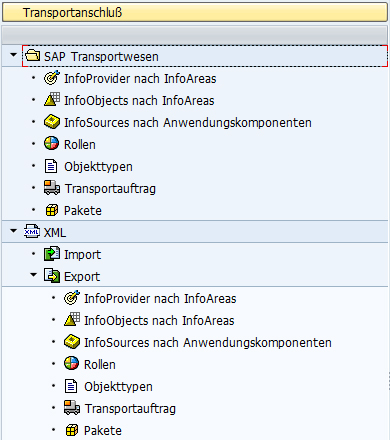
\includegraphics[width=0.55\textwidth]{files/Transportanschluss}
    \caption{Das Transportanschluss Menü}
    \label{pic:Transportanschluss}
\end{figure}
\item[Dokumente:] Zu jedem BI-Objekt können jeweils ein oder mehrere Dokumente in verschiedenen Formaten, Versionen und Sprachen hinzugefügt, verlinkt und durchsucht werden. Diese Dokumente sind in drei Klassen unterteilt und können jeweils \textit{Metadaten}, \textit{Stammdaten} oder \textit{InfoProvider-Daten} zugeordnet werden.
Die Grafische Oberfläche ist in  \textbf{Abb. \ref{pic:Dokumente}}  zu sehen.
\begin{figure}[H]
    \centering
    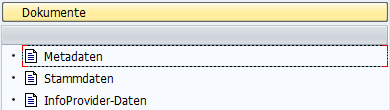
\includegraphics[width=0.6\textwidth]{files/Dokumente}
    \caption{Das Dokumente Menü}
    \label{pic:Dokumente}
\end{figure}
\item[Übersetzung:] Um eine Internationalisierung umsetzen zu können, können mit Hilfe des Moduls \textit{Übersetzung} die Kurz- und Langtexte von BI-Metadaten-Objekten vereinfacht übersetzt werden. Zusätzlich kann die Übersetzungsumgebung, die der SAP Web Application Server (ABAP) beinhalted, verwendet werden.
Die Grafische Oberfläche ist in \textbf{Abb. \ref{pic:Uebersetzung}} zu sehen.
\begin{figure}[H]
    \centering
    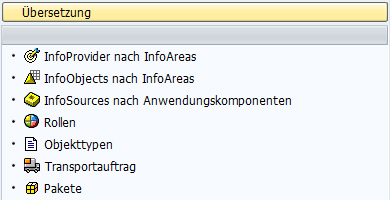
\includegraphics[width=0.6\textwidth]{files/Uebersetzung}
    \caption{Das Übersetzungsmenü}
    \label{pic:Uebersetzung}
\end{figure}
\item[Metadata Repository:] Das Metadata Repository basiert auf HTML und ermöglicht einen zentralen Zugriff auf Informationen von Metadaten-Objekten. Zu diesen Metadaten gehören zum Beispiel wichtige Eigenschaften der Objekte und die Verknüpfungen mit anderen Objekten.
\end{description}




